\documentclass[11pt, spanish]{article}
\usepackage[spanish]{babel}
\selectlanguage{spanish}
\usepackage[utf8]{inputenc}
\usepackage{amsmath}
\usepackage{newfloat}
%\usepackage{fullpage}
\usepackage[top=0.80in, bottom=0.80in, left=0.85in, right=0.85in]{geometry}
\usepackage{multicol}
\usepackage{wrapfig}
\usepackage{enumerate}
\usepackage{graphicx}
\usepackage{newfloat}
\usepackage{geometry}
\usepackage{array}
\usepackage{hyperref}
\usepackage{multirow}
\usepackage{multicol}
\usepackage{float}
\restylefloat{table}
\begin{document}
\title{Ejercitación QGIS}


\thispagestyle{empty}
\begin{center}
	
\includegraphics[width=10cm]{Universidad_San_Andres_UdeSA.jpg}
		
\end{center}
	
	\begin{center}
	\LARGE
\textbf{HERRAMIENTAS COMPUTACIONALES PARA INVESTIGACIÓN}
	

	\vspace{2cm}
	\LARGE
	\textit{Tarea QGIS}

	\vspace{2cm}
	\Large
	Clara Pasman \& Rosario Podestá\
	
	\vspace{1.3cm}
	\Large	
	Profesora: Amelia Gibbons\

	
	\vspace{1.3cm}
	\normalsize
	\today
	\end{center}
	
\clearpage
\section{Base Airbnb Chicago}
\indent Con la idea de obtener un paneo general de la situación socioeconómica y turística de Chicago decidimos analizar el nivel de pobreza, la cantidad de robos, y el precio de alquiler de alojamientos a nivel de comunidad. 


\begin{figure}[hbtp]
\caption{Nivel de pobreza por comunidad}
\centering
\includegraphics[width=12cm]{Pob.jpg}
\end{figure}

\indent Con los datos areales disponibles, logramos representar el nivel de pobreza de un conjunto de barrios que corresponden a una comunidad en particular. Estos conforman un mapa coroplético, el cual describe variables discretas para un subconjunto espacial, en este caso el nivel de pobreza para una comunidad. De manera ilustrativa, la comunidad de Rogers Park tiene entre 32\% y 60\% de hogares bajo el umbral de pobreza. La intensidad de las tonalidades de cada comunidad es creciente, correspondiente a mayores niveles de pobreza. Las comunidades en tonos grises son aquellas para las cuales no se encuentra información disponible.\\ 

\indent Además utilizamos el siguiente histograma para tener una idea más clara sobre la cantidad de comunidades pertenecientes a cada categoría. Es necesario aclarar que el criterio del número de categorías es completamente arbitrario, queda en manos del investigador. 

\begin{figure}[hbtp]
\caption{Nivel de pobreza por comunidad}
\centering
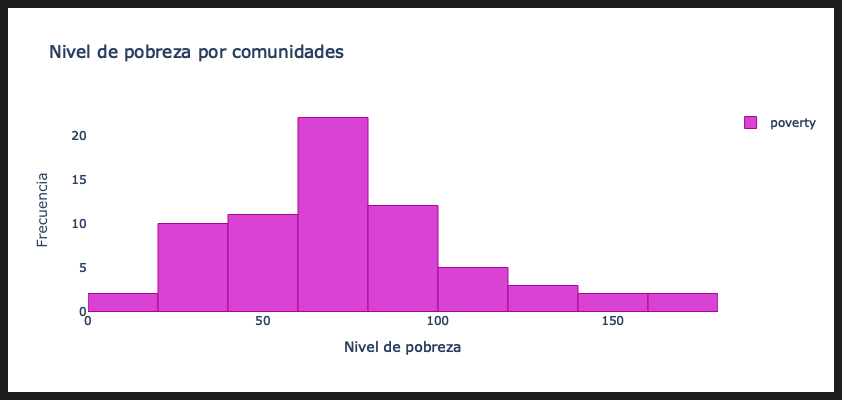
\includegraphics[width=12cm]{Pobgra1.jpg}
\end{figure}

\indent Cada barra indica la frecuencia, la cantidad de comunidades, para cada nivel de pobreza. Observamos una mayor concentración de comunidades con un nivel medio de pobreza, relativos a los valores presentados. La baja frecuencia en los niveles más altos de pobreza sugieren que pocas comunidades son gravemente pobres en Chicago. 
\clearpage

\indent Por otra parte, obtuvimos el número de robos por comunidad. En este caso el mapa coroplético muestra 6 categorías que representan las distintas cantidades de robos en cada area. 

\begin{figure}[hbtp]
\caption{Número de robos por comunidad}
\centering
\includegraphics[width=12cm]{Rob.jpg}
\end{figure}
\clearpage

\indent Nuevamente, también representamos los resultados obtenidos que permite clarificar lo representado en el mapa. 


\begin{figure}[hbtp]
\caption{Número de robos por comunidad}
\centering
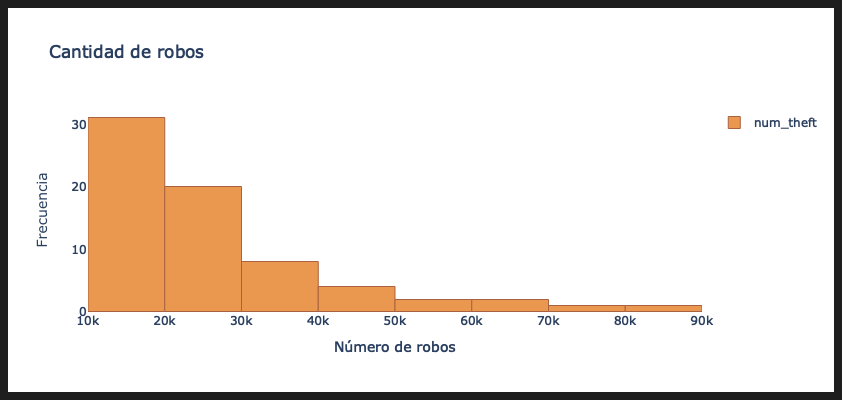
\includegraphics[width=12cm]{Robgra.jpg}
\end{figure}


\indent Podemos observar que la cantidad de comunidades decae a medida que aumenta el número de robos. Podríamos afirmar que el gran porcentaje de este subconjunto de comunidades de Chicago presenta bajos niveles de robos. 
Esto podría vincularse con la alta frecuencia en los niveles bajos y medios de pobreza, lo que podría inducir al turismo en la mayor parte de las comunidades de la ciudad. 

\indent La relación entre estas dos variables se puede ver en el siguiente gráfico. Este explica la frecuencia de niveles de pobreza y número de robos, y permite entrever la cantidad de comunidades con gran números de robos y mucha pobreza, casos contrarios, o intermedios. La información que brinda el gráfico sugiere que las comunidades más pobres presentan mayor número de robos, mientras que la pobreza a niveles medio no se ve estrechamente ligada a número de robos promedio. 

\begin{figure}[hbtp]
\caption{Nivel de pobreza y Número de robos por comunidad}
\centering
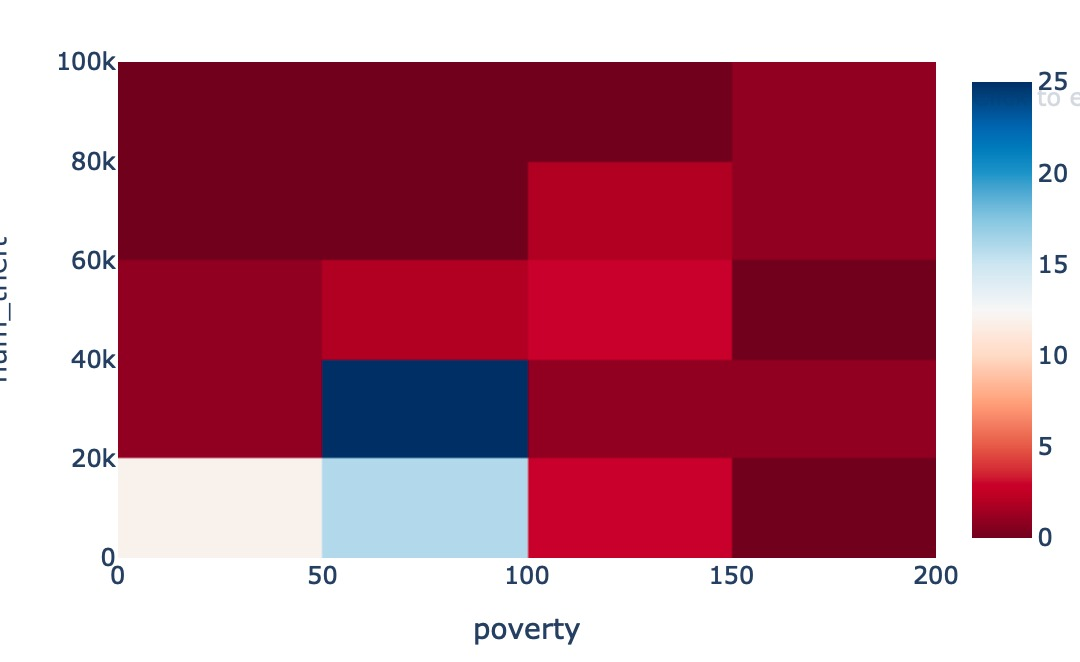
\includegraphics[width=12cm]{pobrob.jpg}
\end{figure}

\indent La última variable elegida es el precio promedio de los alquileres de alojamientos temporales o turísticos. Esta variable también se mide a nivel comunidad, con lo cual también se verá representada en un mapa coroplético. Para remarcar el punto de arbitrareidad con respecto a la cantidad de categorías, en este caso elegimos dividir al rango de precios de alquileres en 7. Lo podemos ver en la siguiente figura.\\

\begin{figure}[hbtp]
\caption{Precios promedio de alojamientos}
\centering
\includegraphics[width=12cm]{Precios.jpg}
\end{figure}

\indent También incluímos el histograma que acompaña al mapa. En este caso, las comunidades por nivel de precios son ascendentes. Esto implica que la gran mayoría de las comunidades alquila sus alojamientos a precios mayores que el promedio, aproximadamente entre 90 y 100 por noche.

\begin{figure}[hbtp]
\caption{Precios promedio de alojamientos}
\centering
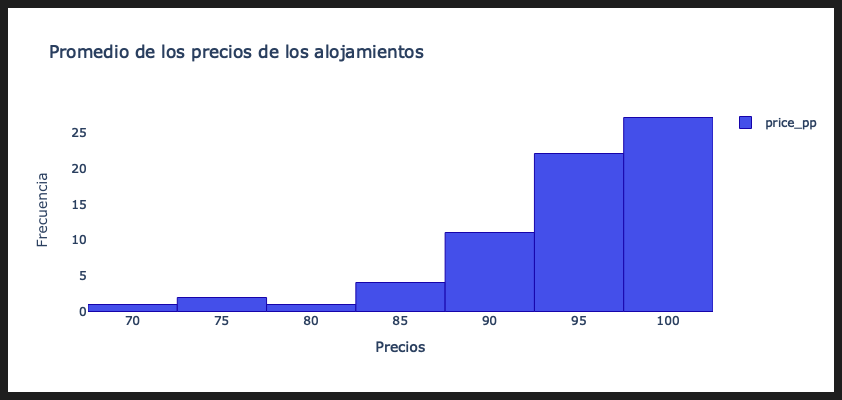
\includegraphics[width=12cm]{Pregra.jpg}
\end{figure}

\indent Las siguientes dos figuras reflejan la relación entre el precio promedio de los alojamientos y el nivel de pobreza, y número de robos respectivamente. Las comunidades con niveles medios de pobreza, y bajo número de robos cobrarán precios más altos. En especial, las comunidades menos pobres y menos inseguras presentarán los mayores niveles de precios. Mientras que aquellas con mayor nivel de pobreza y mayores robos cobrarán menores precios. 

\begin{figure}[hbtp]
\caption{Nivel de Pobreza y Precios promedio de alojamientos}
\centering
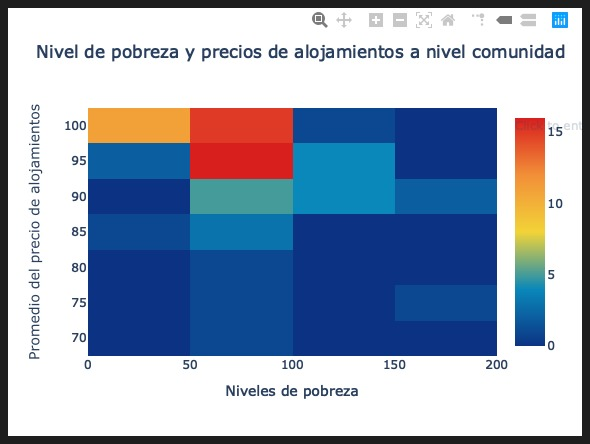
\includegraphics[width=12cm]{Pobpre.jpg}
\end{figure}

\begin{figure}[hbtp]
\caption{Número de Robos y Precios promedio de alojamientos}
\centering
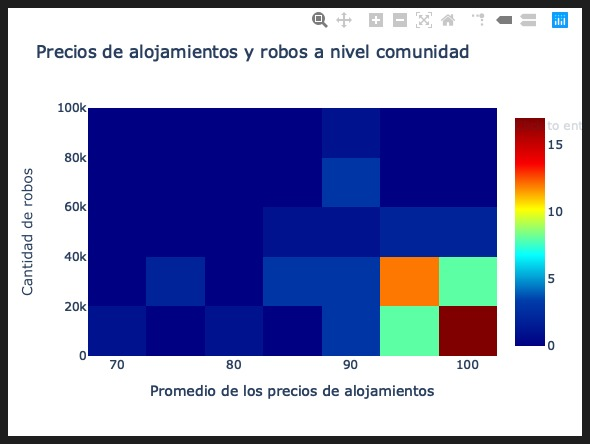
\includegraphics[width=12cm]{Robpre.jpg}
\end{figure}
\clearpage

\section{Base INDEC}
\indent El siguiente mapa muestra los departamentos de la provincia de Buenos Aires  cuya población no alcanza, en promedio, a cubrir determinadas necesidades básicas, y la Ciudad Autónoma de Buenos Aires. En indicador de Necesidades Básicas Insatisfechas (NBI) suele ser utilizado como un proxy de nivel de pobreza, ya que mide la cantidad de necesidades básicas no cubiertas por los hogares. Se observa que en el centro y al oeste de la provincia y en CABA, los hogares logran cubrir sus necesidades relativamente al resto de los departamentos. Observamos una gran concentración de necesidades básicas insatisfechas en el área del Gran Buenos Aires, donde se encuentran los principales asentamientos de la provincia. 
Observamos que la costa presenta mayores niveles de NBI. Esto podría relacionarse con el tipo de actividad económica que se practica en dichas áreas. Las cuales fomentan el desarrollo de grandes ciudades, y consigo de la pobreza. Mientras que el interior, generlamente dedicado a actividades agropecuarias no fomentan la construcción de asentamientos donde el hacinamiento suele ser común.\\ 

\begin{figure}[hbtp]
\caption{Nivel de Necesidades Básicas Insatisfechas por departamento }
\centering
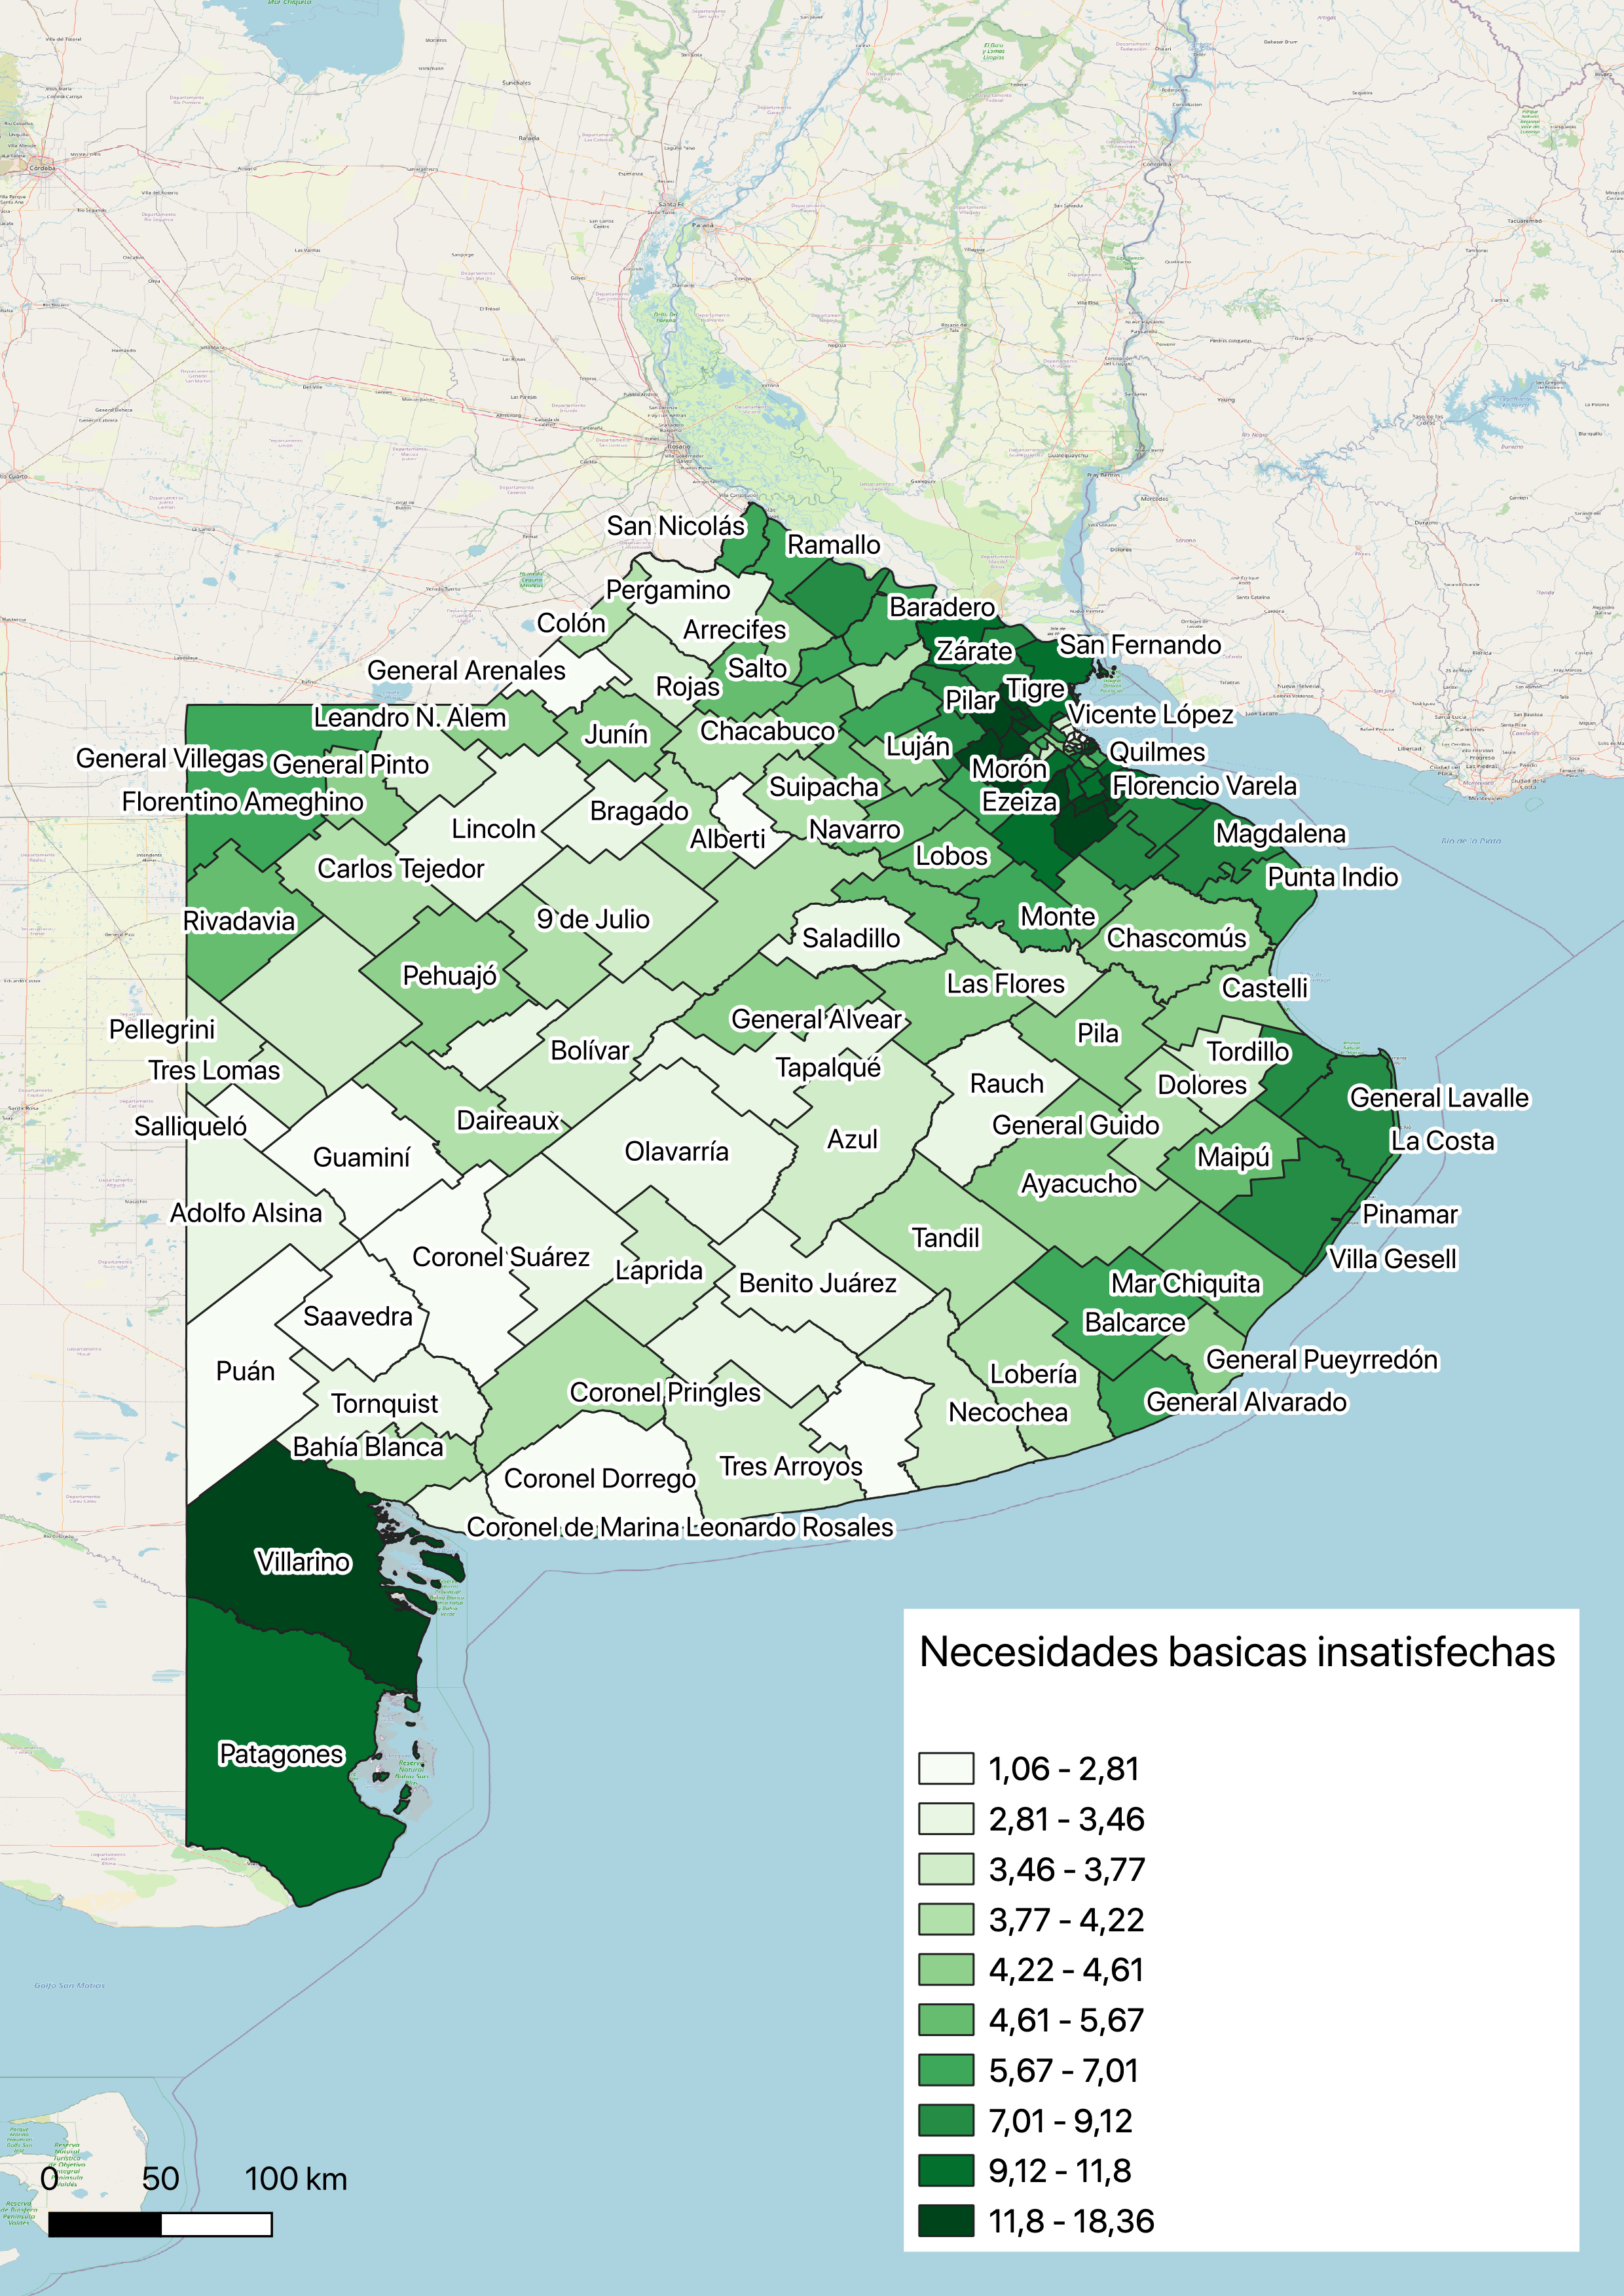
\includegraphics[width=11cm]{NBI.jpg}
\end{figure}

\indent La figura presenta nuevamente a la provincia de Buenos Aires dividida en departamentos y la Ciudad Autónoma de Buenos Aires. En este caso las intensidades de tonalidades representan el nivel de actividad económica de cada departamento. Observamos que el centro y el este de la provincia presentan menores niveles de ocupación, mientras que la costa, en especial el Gran Buenos Aires, CABA y el noreste de la provincia, presentan mayores niveles. Coincidente con el argumento vinculado con las NBI, El acceso al Río de la Plata puede significar un mayor desarrollo económico, ciudades más grandes, y mayores niveles de ocupación. Mientras que en el resto de la provincia relativamente no impulsa altos niveles de ocupación, dada su especialización en el agro. 

\begin{figure}[hbtp]
\caption{Nivel de Actividad Económica por departamento }
\centering
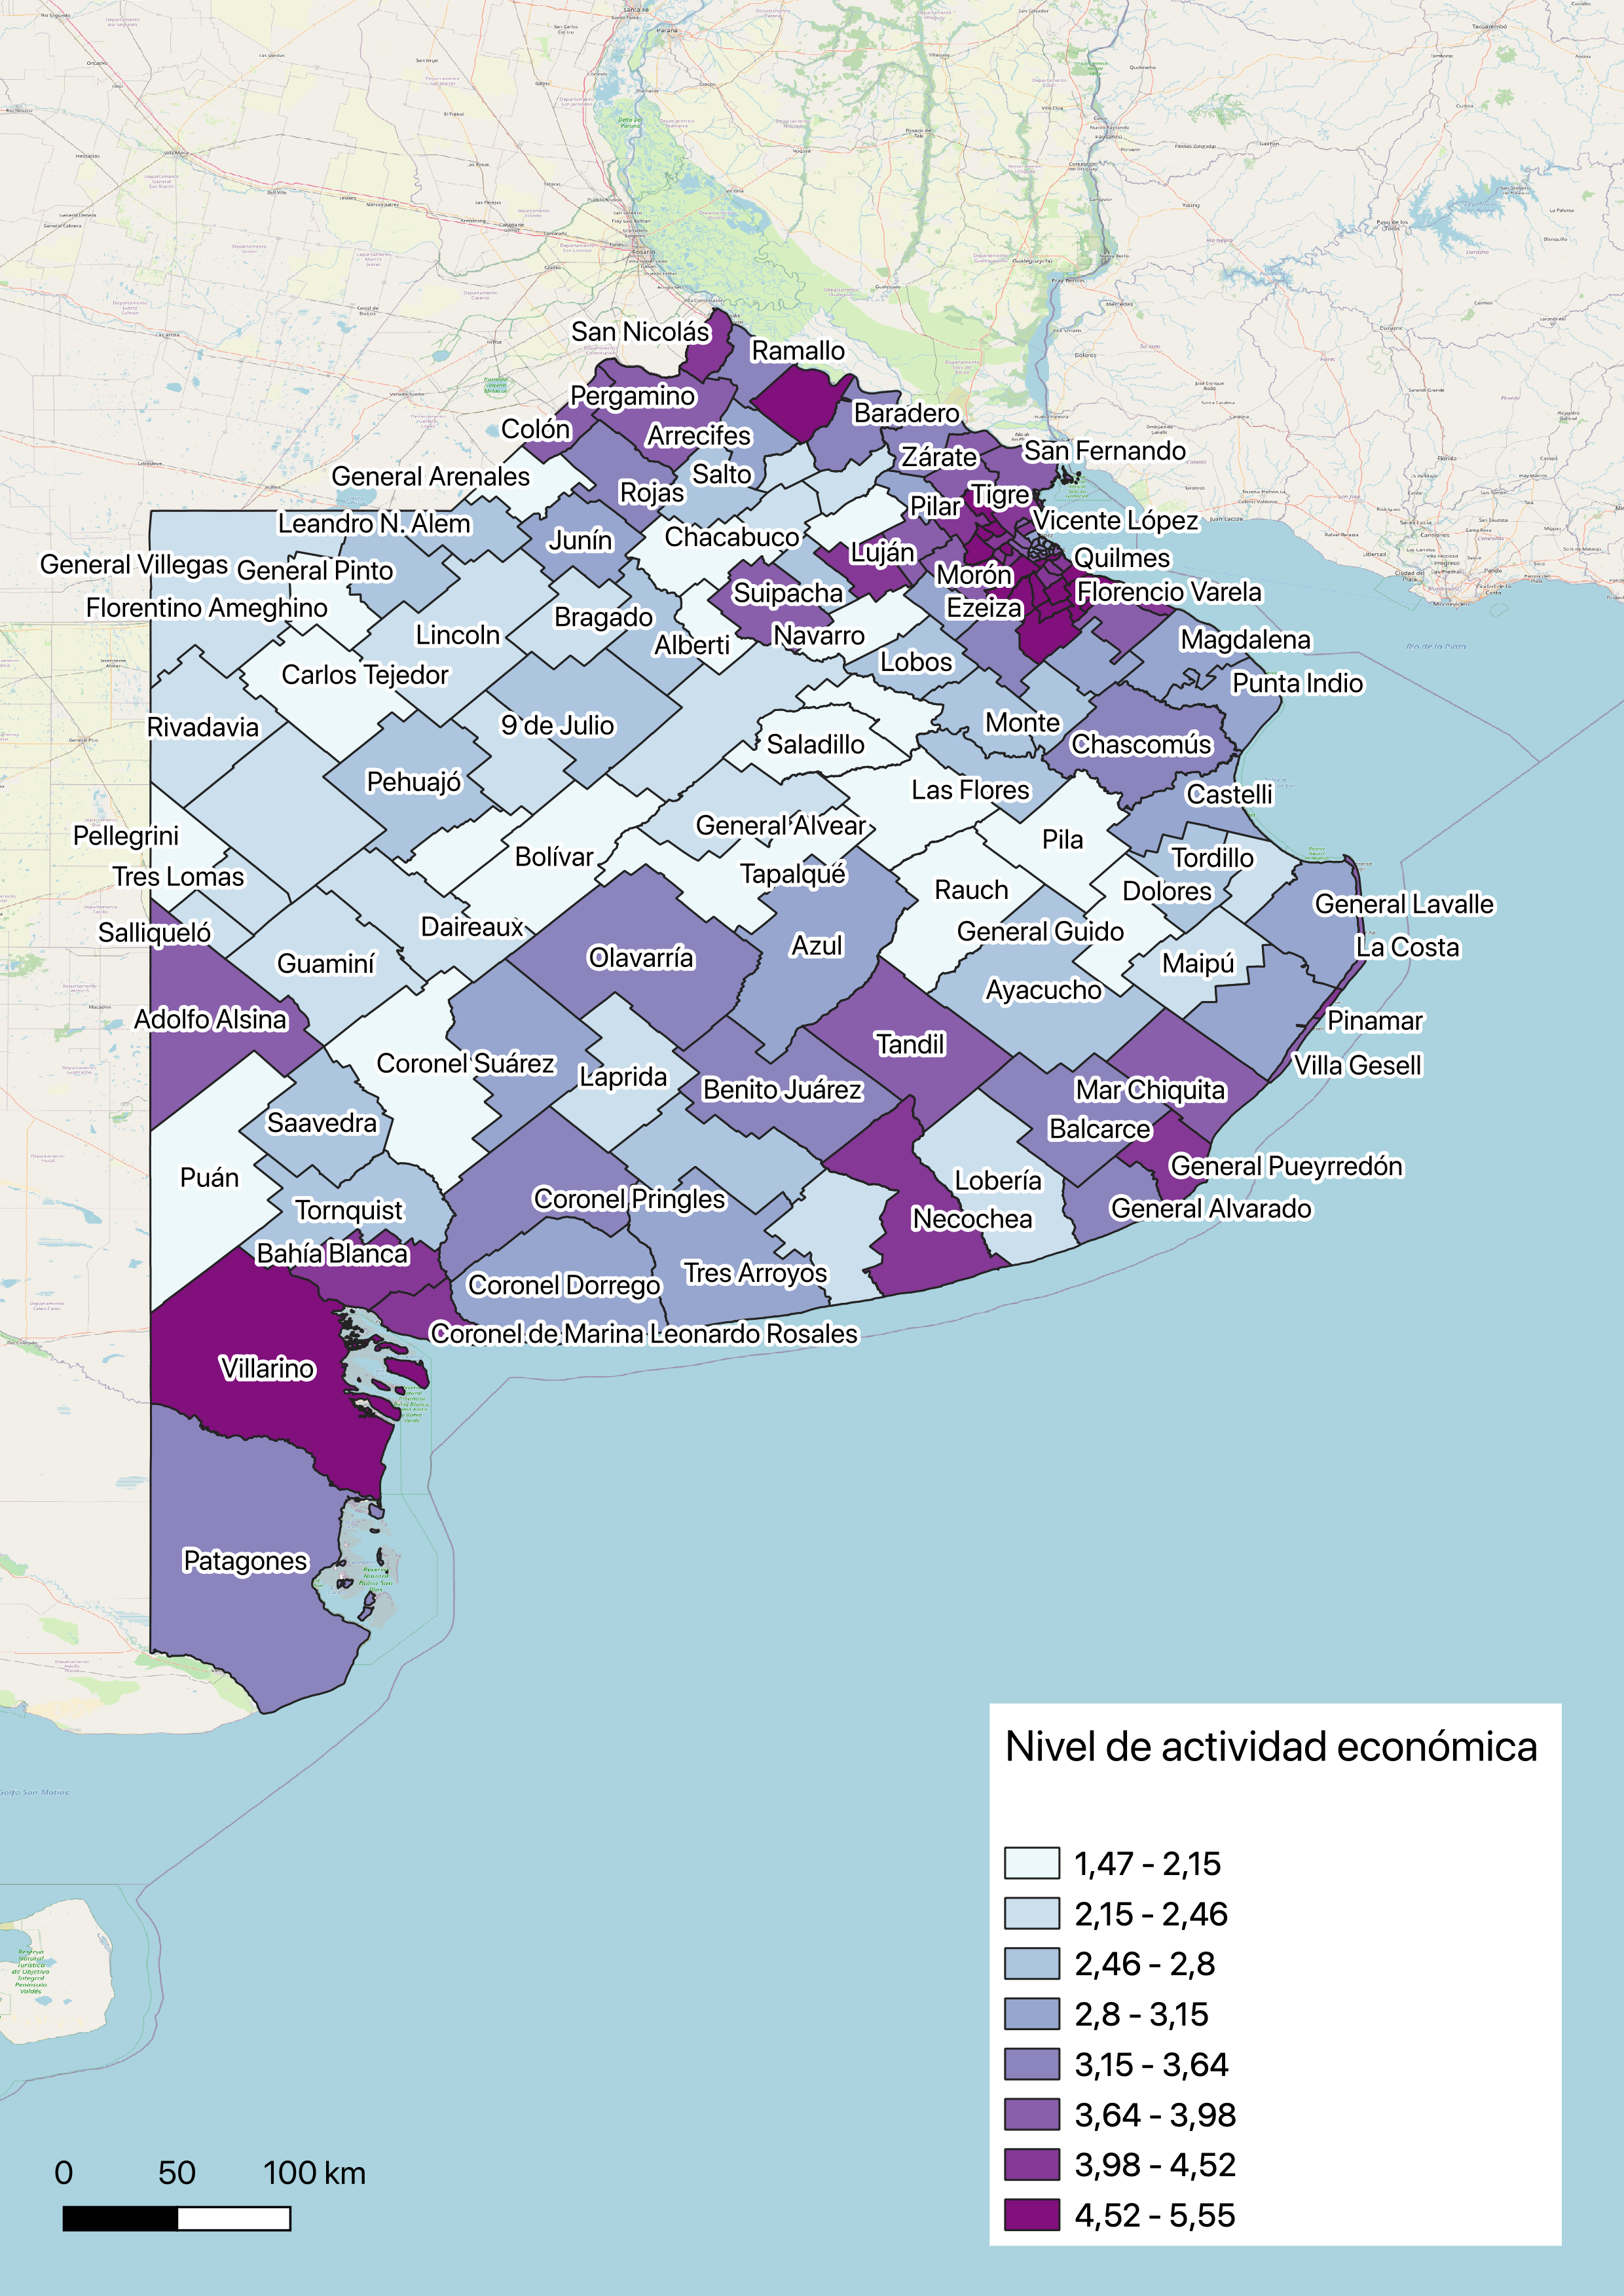
\includegraphics[width=11cm]{Act.jpg}
\end{figure}

\end{document}